%-----------------------------------------------------------------------------------------------%
%
% % Oktober 2022
% Template Latex untuk Laporan Kerja Praktek Program Studi Sistem informasi ini
% Dikembangkan oleh Daffa Takratama Savra (daffatakratama13@gmail.com)

% Template ini dikembangkan dari template yang dibuat oleh Inggih Permana (inggihjava@gmail.com).

% Orang yang cerdas adalah orang yang paling banyak mengingat kematian.
%
%-----------------------------------------------------------------------------------------------%


%-----------------------------------------------------------------------------%
\chapter{\babTiga}
%-----------------------------------------------------------------------------%
\section{Waktu dan Tempat Pelaksaan Kerja Praktek}
Adapun waktu dan tempat pelaksanaan kegiatan kerja praktek ini adalah sebagai berikut:
\par Tanggal           : 01 September 2024 – 30 September 2024 
\par Waktu Kerja    : Senin – Jum’at (08.00 – 15.00)
\par Tempat            : Perumahan Kamala Permai


%-----------------------------------------------------------------------------%
\subsection{Jadwal Kerja Praktek}
Berikut adalah jadwal pelaksanaan kerja praktek ini terhitung 1 bulan (30 hari), seperti pada tabel 3.1 dibawah ini:
%-----------------------------------------------------------------------------%

\begin{table}[H]
\centering
\captionsetup{position=above} % Menempatkan caption di atas tabel
\caption{Jadwal Kerja Praktek}
\begin{tabular}{|c|c|c|c|c|}
\hline
\multirow{2}{*}{\textbf{Jenis Kegiatan}} & \multicolumn{4}{c|}{\textbf{Minggu Ke-}} \\ \cline{2-5} 
                                         & \textbf{I} & \textbf{II} & \textbf{III} & \textbf{IV} \\ \hline
Pengenalan dengan lingkungan kerja        & \cellcolor[HTML]{3166FF} & \cellcolor[HTML]{FFFFFF} & \cellcolor[HTML]{FFFFFF} & \cellcolor[HTML]{FFFFFF} \\ \hline
Pengumpulan data                          & \cellcolor[HTML]{3166FF} & \cellcolor[HTML]{3166FF} & \cellcolor[HTML]{FFFFFF} & \cellcolor[HTML]{FFFFFF} \\ \hline
Analisa dan perancangan sistem            & \cellcolor[HTML]{FFFFFF} & \cellcolor[HTML]{3166FF} & \cellcolor[HTML]{3166FF} & \cellcolor[HTML]{FFFFFF} \\ \hline
Implementasi sistem                       & \cellcolor[HTML]{FFFFFF} & \cellcolor[HTML]{FFFFFF} & \cellcolor[HTML]{3166FF} & \cellcolor[HTML]{3166FF} \\ \hline
Penyusunan laporan                        & \cellcolor[HTML]{FFFFFF} & \cellcolor[HTML]{FFFFFF} & \cellcolor[HTML]{FFFFFF} & \cellcolor[HTML]{3166FF} \\ \hline
\end{tabular}
\end{table}

\subsection{Uraian Kerja Praktek}
%-----------------------------------------------------------------------------%
Tugas Kerja Praktek ini dikerjakan di Perumahan Kamela Permai yang beralamatkan di Taluk Kuantan, Kec. Kuantan Tengah, Kab. Kuantan Singingi dalam kurun waktu 30 hari dihitung sejak 1 September s/d 31 September 2024. Kegiatan yang dilakukan disusun dalam proses perencanaan kerja, rencana tersebut adalah:
\begin{enumerate}
    \item Kegiatan pada minggu pertama dilakukan agenda proses perkenalan dengan tempat kerja. Perkenalan dilakukan pada tanggal 1 September 2024 mulai dari memperkenalkan diri kepada para pegawai. Perkenalan ini juga sekaligus berlangsung dengan pengumpulan data, yaitu dengan melakukan teknik pengumpulan seperti observasi dan wawancara.
    \item Pada Minggu kedua dilakukan proses pengamatan alur dan prosedur kerja, identifikasi tugas, khususnya di bidang bagian umum. Sekaligus memulai untuk menganalisa serta merancang sistem yang akan dibuat.
    \item  Pada minggu ketiga dilakukannya pengimplementasian sistem bersama pihak instansi.
    \item  Selanjutnya pada minggu keempat yaitu melakukan penyusunan laporan yang berasal dari data yang sudah diperoleh.
\end{enumerate}
%-----------------------------------------------------------------------------%
\section{Menentukan Data Yang Diperlukan}
\par Adapun data yang dikumpulkan pada saat kerja praktek adalah sebagai berikut:

\begin{enumerate} [label=\alph*.]
\item Data Primer
\par Data Primer adalah data yang diambil secara langsung dari sumber aslinya, melalui narasumber yang tepat dan dapat dijadikan data pembuatan laporan. Data primer tersebut adalah:
	\begin {enumerate}
	\item Daftar harga rumah setiap tipenya.
	\item Lokasi dan \textit{siteplan} untuk membuat visual digital
	\end{enumerate}
\item Sekunder
\par Data Sekunder adalah data yang diambil melalui jurnal, e-book dan juga buku-buku referensi dari berbagai penulis.
\end{enumerate}
%-----------------------------------------------------------------------------%
%-----------------------------------------------------------------------------%
\section{Metodologi Kerja Praktek}
%-----------------------------------------------------------------------------%
\begin{figure}
    \centering
    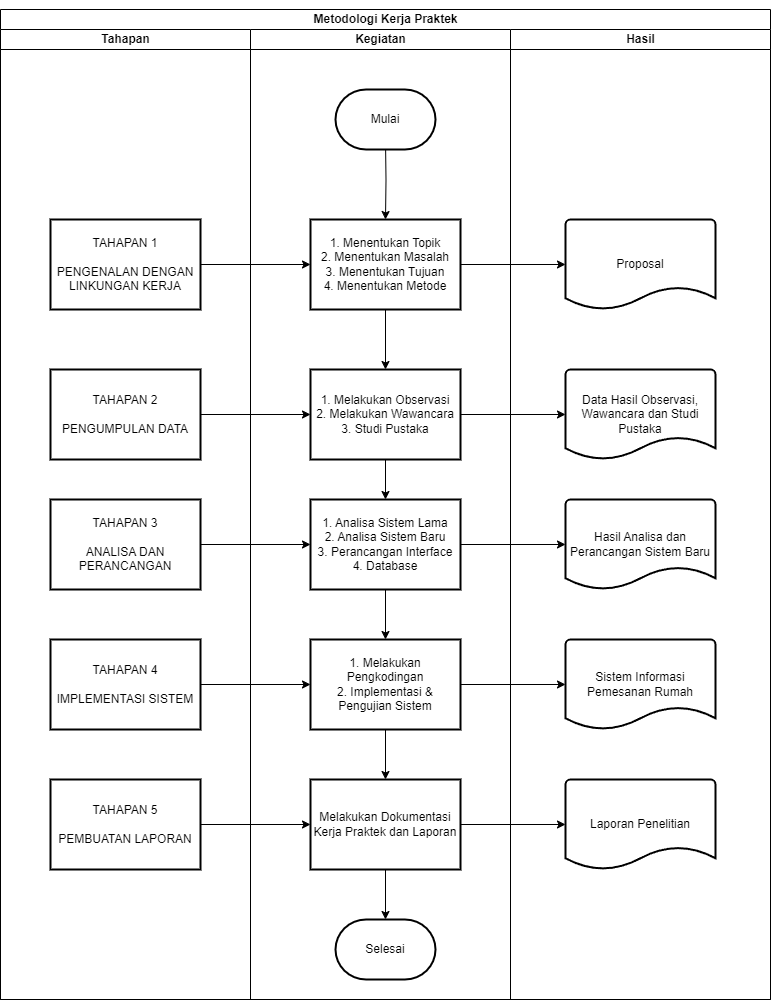
\includegraphics[width=\textwidth]{Flowchart Metodologi Kerja Praktek.png}
    \caption{Metodologi Kerja Praktek}
    \label{fig:enter-label}
\end{figure}
%-----------------------------------------------------------------------------%
\subsection{Tahap Pengenalan dengan Lingkungan Kerja}
%-----------------------------------------------------------------------------%
\par Langkah Pertama adalah perkenalan dengan lingkungan instansi sekaligus menetapkan masalah yang akan dipecahkan dalam instansi tersebut. Adapun langkah-langkah dalam tahap ini adalah sebagai berikut:

\begin{enumerate}
    \item Mulai\\Merupakan tahapan awal dalam setiap kegiatan yang akan dilakukan. 
    \item Menentukan Topik Penelitian\\Topik penelitian ditentukan dari uraian masalah dan kendala yang didapat dari observasi secara langsung di Perumahan Kamela Permai.
 \item Menentukan Masalah\\Setelah observasi dilakukan untuk mendukung pencapaian kerja praktek maka selanjutnya dilakukan penentuan masalah agar bisa mendapat masalah yang lebih fokus untuk dipecahkan. 
    \item Menentukan Tujuan Kerja Praktek\\Selanjutnya adalah penentuan tujuan dari kerja praktek ini agar tujuan dalam penulisan Laporan Kerja Praktek lebih Jelas. 
 \item Menentukan Metode Penelitian\\Agar hasil dari penelitian ini sesuai harapan maka dibutuhkan penentuan metode penelitian untuk mendukung penelitian ini. 
\end{enumerate}
%-----------------------------------------------------------------------------%
\subsection{Tahap Pengumpulan Data}
%-----------------------------------------------------------------------------%
\par Tahap ini adalah tahap penulis melaksanakan Kerja Praktek, pada tahap ini yang dilakukan adalah:

\begin{enumerate}
    \item Observasi\\Penulis melakukan pengamatan di Perumahan Kamela Permai secara langsung juga melakukan peninjauan di Perumahan Kamela Permai. 
    \item Wawancara\\Penulis melakukan wawancara langsung dengan marketing Perumahan Kamela Permai terkait pemesanan perumahan. 
    \item Studi Pustaka\\Studi Pustaka dilakukan dengan cara mengambil literature yang berkaitan dengan materi. Pada tahapan pengumpulan data studi pustaka penulis mengambil beberapa referensi dari buku, jurnal, e-book dan internet.
\end{enumerate}
%-----------------------------------------------------------------------------%
\subsection{Tahap Analisa dan Perancangan}
%-----------------------------------------------------------------------------%
\par Beberapa hal yang perlu dilakukan dalam tahap analisa dan perancangan sistem adalah sebagai berikut:

\begin{enumerate}
	    \item Analisa Sistem Lama\\Pada tahap analisa sistem lama atau sistem yang berjalan, penulis melihat langsung bagaimana proses pemesanan berlangsung dimana calon pembeli akan datang ke kantor pemasaran dan merencanakan pemesanan serta menanyakana dokumen yang perlu disiapkan. 
	    \item Analisa Sistem Baru\\Pada tahap analisa sistem baru penulis mengambil usulan berdasarkan masalah dan kendala yang sudah dilakukan di analisa sistem yang berjalan (sistem lama), sehingga penulis mempunyai usulan sistem baru berupa:
			\begin{enumerate} 
			\item Penyimpanan data setiap rumah beserta type dan harganya menggunakan database
			\item Pencarian data untuk mengurangi penumpukan data.
			\end{enumerate}
	    \item Perancangan \textit{Interface}\\Pada tahap ini penulis membuat perencangan interface yang merupakan desain dari fitur yang telah diusulkan pada analisa sistem baru yang menghasilkan perancangan sebagai berikut:
	\begin{enumerate} [label=\alph*.]
		\item Perancangan \textit{interface} halaman \textit{home}.
		\item Perancangan \textit{interface} halaman \textit{siteplan} untuk pemesanan.
		\item Perancangan \textit{interface} halaman data rumah.
		\item Perancangan \textit{interface} halaman data pengunjung.
		\item Perancangan \textit{interface} halaman panduan pemesanan.
		\item Perancangan \textit{interface} halaman \textit{gallery}.
		\item Perancangan \textit{interface} halaman harga.
		\item Perancangan \textit{interface} halaman kontak.
		\item Perancangan \textit{interface} halaman \textit{login}
		\item Perancangan \textit{interface} halaman \textit{booking}
		\item Perancangan \textit{interface} halaman \textit{Dashboard}
	\end{enumerate}
	\item \textit{Database}\\Pada tahap ini penulis melakukan rancangan database berdasarkan perancangan interface yang telah ditentukan yaitu membuat struktur \textit{tabel, record, field} dan \textit{ERD}.
\end{enumerate}
%-----------------------------------------------------------------------------%
\subsection{Tahap Implementasi}
%-----------------------------------------------------------------------------%
Dalam tahap pembuatan sistem informasi absensi pegawai ini terdapat pengodingan dan pendesain web. Yaitu dengan menggunakan bahasa pemrograman \textit{PHP} dengan menggunakan \textit{HTTP Library Oktaax} dan \textit{MySQL} sebagai \textit{Database}. Implementasi Sistem yaitu tahap dimana sistem siap dioperasikan pada keadaan yang sebenarnya sesuai dari kebutuhan dari perumahan, sehingga dapat diketahui sistem yang dibuat benar-benar dapat memecahkan masalah yang ada.
%-----------------------------------------------------------------------------%
\subsection{Tahap Penulisan Laporan}
%-----------------------------------------------------------------------------%
\par Tahap terakhir adalah melakukan penyusunan laporan. Kegiatan yang dilakukan diantaranya melakukan konsultasi terhadap pembimbing kerja praktek, melakukan dokumentasi hasil kerja praktek, dan selesai.
\par Penelitian sebagai bahan dari laporan kerja praktek ini dilakukan dengan menggunakan penelitian deskriptif yaitu metode penelitian yang bertujuan menggambarkan secara sistematis dan akurat mengenai data-data yang ada dengan cara mengumpulkan dan mengklasifikasikan data yang diperoleh, kemudian dianalisis dengan teori yang telah dipelajari.
%-----------------------------------------------------------------------------%